\section{Evaluation}
\label{sec:evaluation}


We evaluate \tool by implementing a word count program with prior text parsing, TPCH query 12 and a k-means application that uses array processing extension for \tool. \\

All experiments were performed on the Amazon EC2 Cloud, using 20 "m1.large" nodes as slaves and one as master. They each have 7.5 Gb of memory, 2 virtual cores with 2 EC2 compute units each, have 850 Gb of instance storage and provide high throughput. Prior to the experiments we have measured up to 50 MB/s between two nodes. For the Hadoop experiments we used current Clouderas Hadoop distribution cdh3u4. We used Crunch version 0.2.4 and Scoobi 0.4.0. For Spark we used the Mesos \todo{cite} EC2 script to start a cluster, and then used Spark version 048276799 for our tests. We did not tweak Hadoop configuration beyond the default settings. For Spark we changed the default parallelism level to the number of machines in the cluster and increased the available memory to 6GB. 

\todo{Maybe move regex to optimizations}
% Regular expressions
For a fairer comparison with Pig we adapted some of their regex optimizations for our program. Pig makes use of a faster library \todo{cite brics.automaton} and implements an optimized splitting function when the regular expression becomes a simple comparison of one character. We implemented a frontend for regular expressions which automatically selects the best variant for each expression and operation. 

We were also getting unsatisfying numbers from our Scoobi backend, so we added Crunch with about one week of effort. This really shows that it is easy to implement a new backend, and the modularity allows us to reuse pieces of other backends. Crunch's implementation of join performed very badly in local benchmarks, so we replaced it with our own one for these benchmarks.

% Data Serialization
For serialization of data we used LMS code generation to achieve minimal overhead for both Crunch and Scoobi frameworks. We used generated versions since they outperformed the Kryo framework by a thin margin. For Spark we used Kryo. All benchmarks were run three times and in the figures we present only the average. We also measured standard deviation but it is not displayed since it is smaller than 3\% of the job time in all experiments.

\begin{figure}[!hbt]
    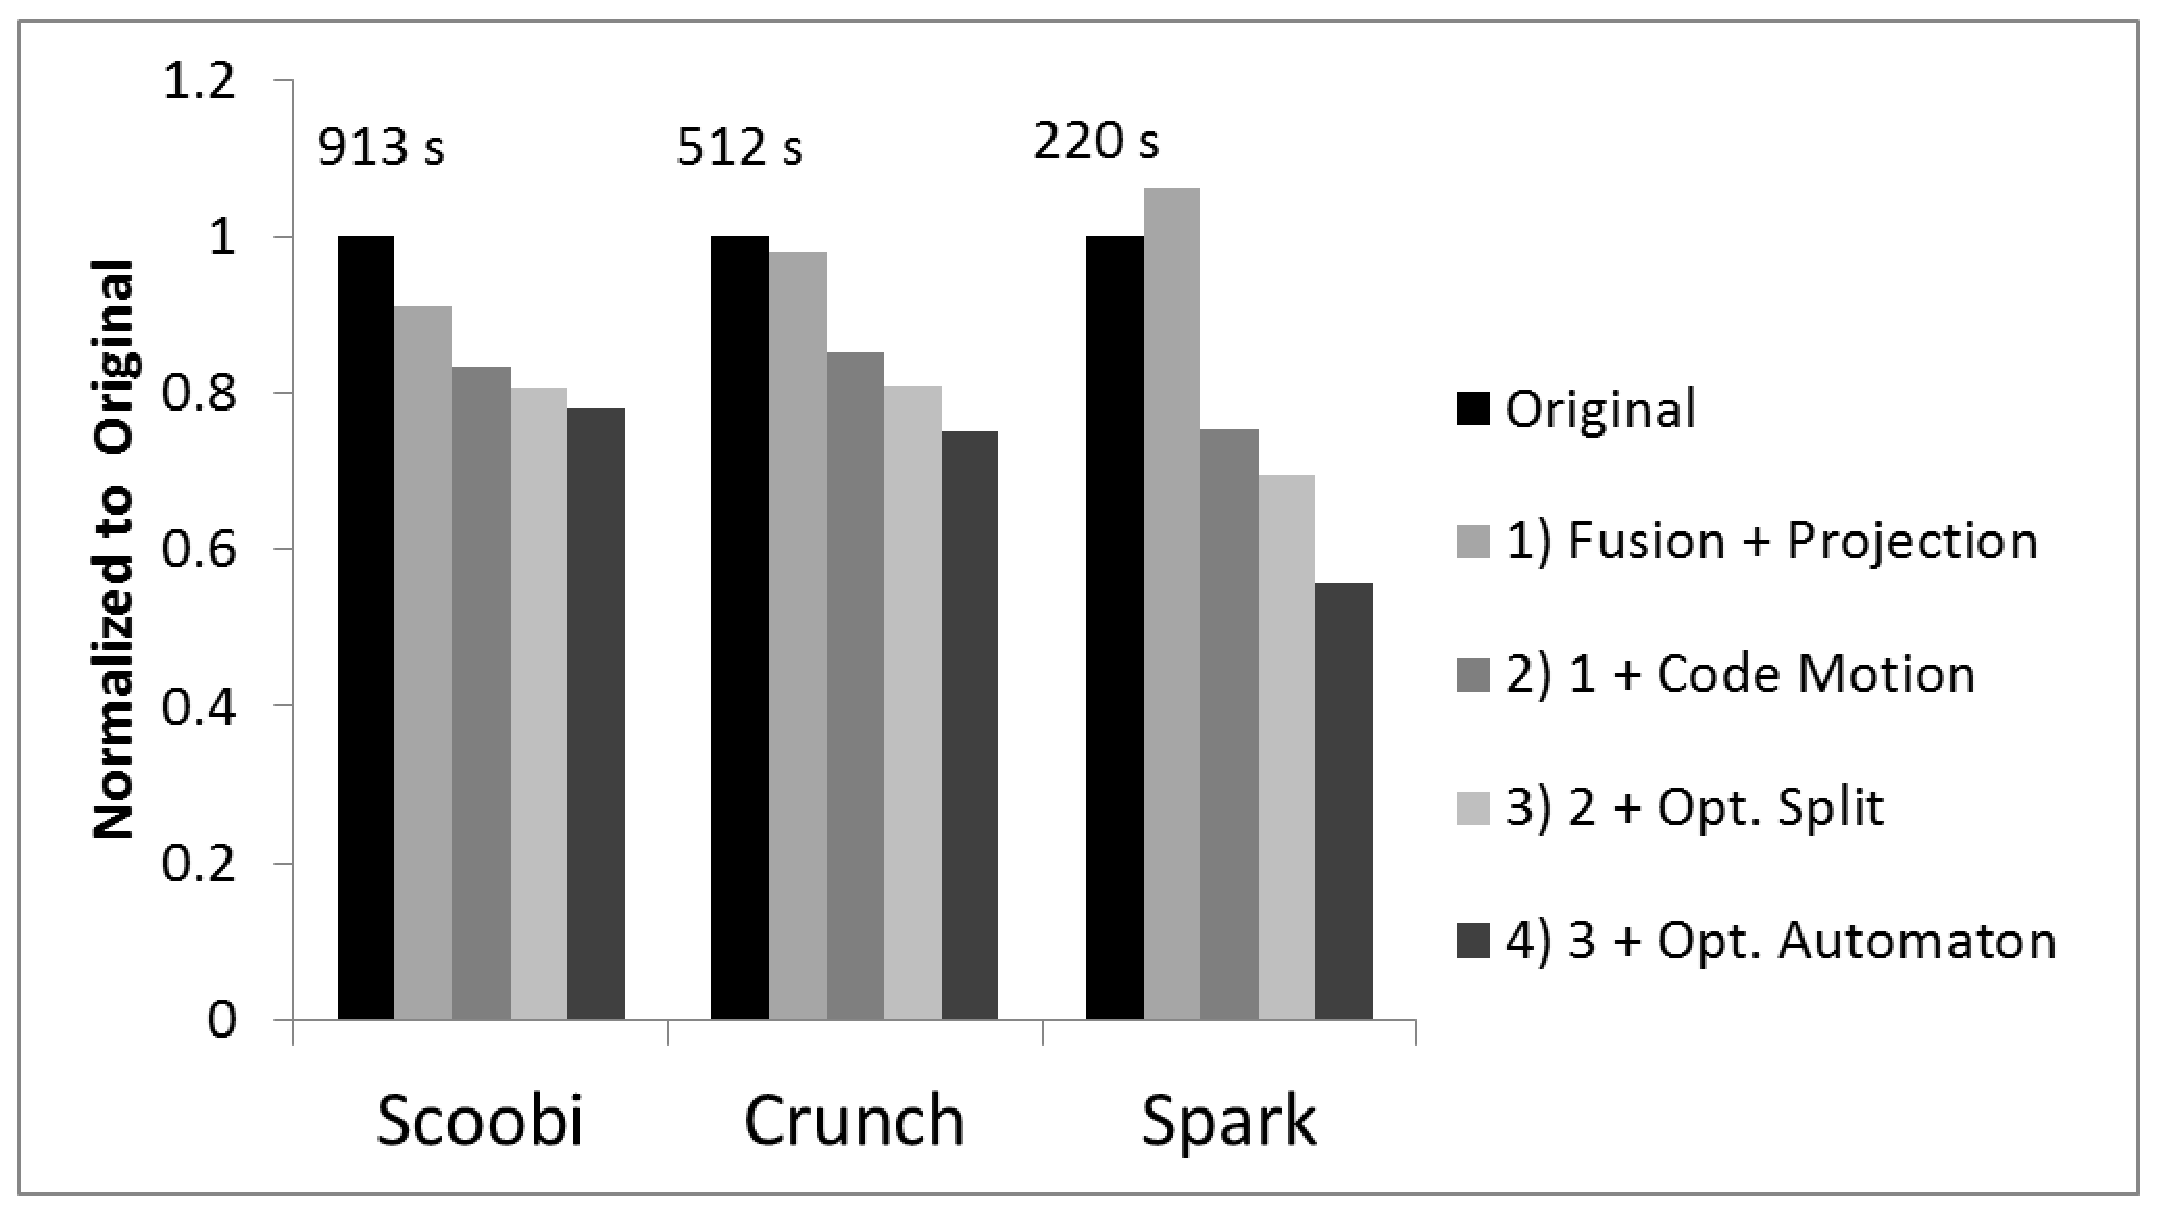
\includegraphics[width=8.6cm]{figures/word-count}
    \label{fig:word-count}\\%\vspace{10pt}
   \caption{KMeans}
\end{figure}

\begin{figure}[!hbt]
    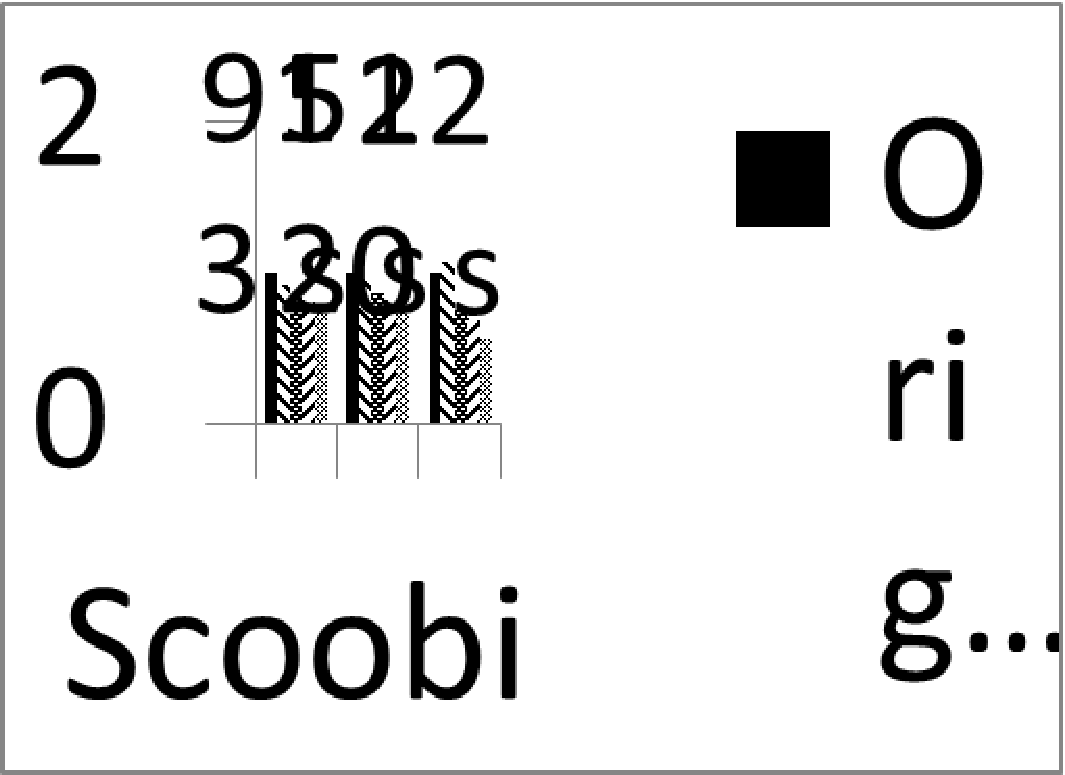
\includegraphics[width=8.6cm]{figures/k-means}
    \label{fig:k-means}\\%\vspace{10pt}
   \caption{KMeans}
\end{figure}

\begin{figure}[!hbt]
    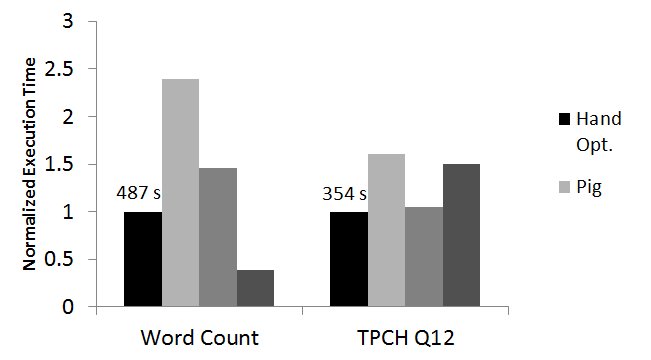
\includegraphics[width=8.6cm]{figures/pig}
    \label{fig:pig}\\%\vspace{10pt}
   \caption{KMeans}
\end{figure}

\begin{figure}[!hbt]
    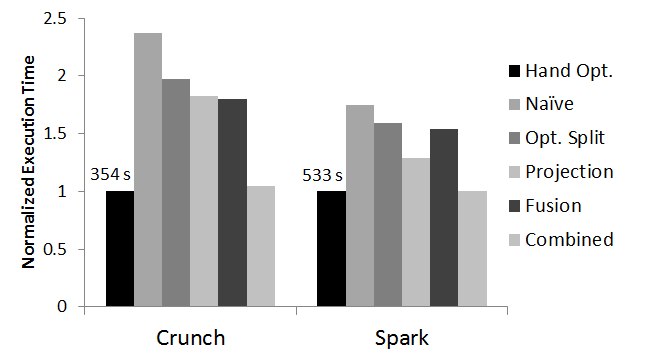
\includegraphics[width=8.6cm]{figures/tpch}
    \label{fig:tpch}\\%\vspace{10pt}
   \caption{KMeans}
\end{figure}

% WordCount
\subsection{Parsing and Word Count}
\label{subsec:parsing-word-count}
\todo{Stivo explain the regular expressions and what do we want to prove}
Our input is a 62 Gb set of freebase wikipedia data. As the data in that example is not entirely cleaned up we use regular expressions to filter out words and to split it in a custom manner. Our program uses 5 regular expressions in total which are quite expensive and we are certain that this is a cpu-bound program, such that our optimizations become relevant.
It can not benefit from field reduction and it only requires one shuffle stage, so its performance is dependant on the cpu time on the mapper side. 

For this evaluation we start with an unoptimized version and add optimizations one by one. We first add our loop fusion and field reduction optimizations. Then we reuse the patterns instead of recompiling them. Next we add the fast splitter and for the fully optimized version we add the faster regex library. 

In figure \todo{\ref{}} we show the job times for these versions normalized to the unoptimized program version. In this benchmark we notice that code motion removes regular expressions automaton compilation from the hot loop. Performance improvements are from \todo{75-82} in Scoobi, \todo{Crunch} and in Spark. Also, we notice significant fusion increase in Scoobi which indicates that the framework imposes additional overhead for declarative operations. 

In Spark, we notice larger benefits from optimizations. We believe that it has significantly smaller IO overhead so that the optimizations have a bigger effect. Also, we notice that fusion optimization and field reduction is slower than the original program, but only in Spark. This result does not match our experiments in a smaller cluster setup. We believe that it could be caused by a straggler node in the cloud environment.

% TPCH q12
\subsection{TPCH Query 12}
\label{subsec:tpch-query-12}

To evaluate effects of projection insertion we have run the TPCH query 12 which includes an expensive \code{join} operation and aggregates the whole result to just two values. As the data set we use a 100 GB input data set generated by \todo{dbgen cite}.

In figure \todo{\ref{}} we show job times for different optimizations normalized to the unoptimized program version. We notice that projection insertion gives \todo{from bla to bla} percent better performance on Crunch and \todo{from bla to bla} for Scoobi. In the figure we also show that projection insertion gives significantly better improvements in Spark than in Hadoop based frameworks. We believe that either network shuffle or the \code{join} operation are less optimal in Spark. \todo{Combined optimizations provide better improvements than a sum of individual ones. We explain that by the compiler optimizations shown in \todo{\ref{}}}.


\subsection{Comparison with Pig}
\label{subsec:pig}
% Pig Comparison

In figure \todo{\ref{}} we compare most optimal versions of benchmarks to equivalent Pig programs. The figure is normalized to the Pig execution time and overall job time is stated above the bar. We notice that for TPCH query 12, combination of fusion, code motion and field reduction outperform Pig when the Crunch framework is used. For Crunch, field reduction alone is not enough to outperform the Pig framework. We believe that this result is caused by more efficient join operation in Pig. In future work we will investigate the cause for this.
In the Word Count Crunch outperforms Pig even without any optimizations applied. With all optimizations the difference is significant. We explain this by the more optimal regular expressions processing support included in \tool. In regular expressions used in the benchmark Pig falls back to default Java regular expressions while \tool uses optimized automaton library. Scoobi framework performs slower than Pig in both benchmarks even with all optimizations applied.

For the sake of showing comparison between the Hadoop based frameworks and the Spark framework we include the Spark results in the graph. We see that in all cases except for unoptimized TPCH query 12 it significantly outperforms Hadoop based frameworks. \todo{include or not?} Spark has a small advantage, as the user is required to copy the program to all machines before running it. Also the Hadoop frameworks need to submit two jobs for TPCH Q12, while spark can start 4 stages with very low latencies.

\subsection{K-Means}
\label{subsec:kmeans}
\todo{Stivo KMeans graph explanation}
% KMeans
We took a version of Sparks Kmeans application and ported it to our own language. This application can neither use field reduction nor can it really profit from loop fusion. We extended our DSL for this program with a highly optimized Vector class, which is compiled into an Array. As this program uses operations only available in spark, and it has been shown that Spark outperforms Hadoop by a large margin for it, we have only benchmarked it against the original Spark implementation. As input we use synthetic data with 10 to 1000 dimensions, 100 centers and we keep the dimensions * points factor constant at 2000000000, such that each input file is around 20Gb. 

Our results are similar to those of Steno: In lower dimensions our optimization shows an impressive speedup while at 1000 dimensions our version performs slightly worse. We believe that the iterator overhead is quite high for 10 dimensions, such that our loops which removes it performs much better. At higher dimensions it's possible that the JVM can do a better job optimizing if the code is smaller, such that our pre optimized and larger code becomes slightly slower. In any case our implementation seems favorable as it performs more consistently for different dimensions.
